\iffalse
\documentclass[12pt]{article}
\usepackage{graphicx}
\usepackage{amsmath}

\begin{document}
\begin{center}
\textbf\large{CHAPTER-7 \\ COORDINATE GEOMETRY}

\end{center}
\section*{Excercise 7.4}
\fi
%\begin{enumerate}[label=\thechapter.\arabic*,ref=\thechapter.\theenumi]
\begin{enumerate}[label=\thesection.\arabic*,ref=\thesection.\theenumi]
\numberwithin{equation}{enumi}
\numberwithin{figure}{enumi}
\numberwithin{table}{enumi}
\item Determine the ratio in which the line $2x+y  - 4=0$ divides the line segment joining the points $\vec{A}(2, - 2)$  and  $\vec{B}(3, 7)$.
\item Find a relation between $x$ and $y$ if the points $(x, y), (1, 2)$  and  $(7, 0)$ are collinear.

\item Find the centre of a circle passing through the points $(6, – 6), (3, – 7)$ and $ (3, 3)$.

\item The two opposite vertices of a square are $(–1, 2)$  and $ (3, 2)$. Find the coordinates of the other two vertices.

\iffalse
\item The Class X students of a secondary school in Krishinagar have been allotted a rectangular plot of land for their gardening activity. Sapling of Gulmohar are planted on the boundary at a distance of 1m from each other. There is a triangular grassy lawn in the plot as shown in fig.\ref{fig:Fig1}. The students are to sow seeds of flowering plants on the remaining area of the plot.\\

\begin{figure}[!h]
	\begin{center} 
	    \includegraphics[width=\columnwidth]{./ss}
	\end{center}
\caption{}
\label{fig:Fig1}
\end{figure}
\item Taking $\vec{A}$ as origin, find the coordinates of the vertices of the triangle.
\item What will be the coordinates of the vertices of $\triangle PQR$ if $\vec{C}$ is the origin?
Also calculate the areas of the triangles in these cases. What do you observe?
\end{enumerate}

\fi

\item The vertices of a $\triangle ABC$ are $\vec{A}(4,6), \vec{B}(1,5)$ and  $\vec{C}(7,2)$. A line is drawn to intersect sides $AB$ and $AC$ at $\vec{D}$ and $\vec{E}$ respectively, such that $\frac{AD}{AB} = \frac{AE}{AC} = \frac{1}{4}$. Calculate the area of $\triangle ADE$ and compare it with the area of the $\triangle ABC$.

\item Let $\vec{A}(4, 2), \vec{B}(6, 5)$  and $ \vec{C}(1, 4)$ be the vertices of $\triangle ABC$.

\begin{enumerate}
\item The median from $\vec{A}$ meets $BC$ at $\vec{D}$. Find the coordinates of the point $\vec{D}$.
\item Find the coordinates of the point $\vec{P}$ on $AD$ such that $AP : PD = 2 : 1$.
\item Find the coordinates of points $\vec{Q}$ and $\vec{R}$ on medians $BE$ and $CF$ respectively such that $BQ : QE = 2 : 1$  and  $CR : RF = 2 : 1$.
\item What do you observe?
\item If $\vec{A}, \vec{B}$ and $\vec{C}$  are the vertices of $\triangle ABC$, find the coordinates of the centroid of the triangle.
\end{enumerate}


\item $ABCD$ is a rectangle formed by the points $\vec{A}(–1, –1), \vec{B}(– 1, 4), \vec{C}(5, 4)$  and  $\vec{D}(5, – 1)$. $\vec{P}, \vec{Q}, \vec{R}$ and $\vec{S}$ are the mid-points of $AB, BC, CD$ and $DA$ respectively. Is the quadrilateral $PQRS$ a square? a rectangle? or a rhombus? Justify your answer.
	\\
	\iffalse
\documentclass[12pt]{article}
\usepackage{graphicx}
%\documentclass[journal,12pt,twocolumn]{IEEEtran}
\usepackage[none]{hyphenat}
\usepackage{graphicx}
\usepackage{listings}
\usepackage[english]{babel}
\usepackage{graphicx}
\usepackage{caption} 
\usepackage{hyperref}
\usepackage{booktabs}
\usepackage{array}
\usepackage{amsmath}   % for having text in math mode
\usepackage{listings}
\lstset{
  frame=single,
  breaklines=true
}
  
%Following 2 lines were added to remove the blank page at the beginning
\usepackage{atbegshi}% http://ctan.org/pkg/atbegshi
\AtBeginDocument{\AtBeginShipoutNext{\AtBeginShipoutDiscard}}
%


%New macro definitions
\newcommand{\mydet}[1]{\ensuremath{\begin{vmatrix}#1\end{vmatrix}}}
\providecommand{\brak}[1]{\ensuremath{\left(#1\right)}}
\providecommand{\norm}[1]{\left\lVert#1\right\rVert}
\newcommand{\solution}{\noindent \textbf{Solution: }}
\newcommand{\myvec}[1]{\ensuremath{\begin{pmatrix}#1\end{pmatrix}}}
\let\vec\mathbf

\begin{document}

\begin{center}
\title{\textbf{Properties of Quadrilaterals}}
\date{\vspace{-5ex}} %Not to print date automatically
\maketitle
\end{center}

\setcounter{page}{1}



\section{10$^{th}$ Maths - Chapter 7}

This is Problem-8 from Exercise 7.4

\begin{enumerate}
\item ABCD is a rectangle formed by the points $\vec{A}(–1, –1), \vec{B}(– 1, 4), \vec{ C}(5, 4) \text{ and } \vec{D}(5, – 1)$. $\vec{P,Q,R} \text{ and } \vec{S}$ are the mid-points of $\vec{AB, BC, CD} \text{ and } \vec{DA}$ respectively. Is the quadrilateral
PQRS a square? a rectangle? or a rhombus? Justify your answer. \\
\fi
\solution 
See Fig. \ref{fig:10/7/4/8Fig3}.
\begin{align}
  \label{eq:10/7/4/8det2f}
  \vec{P} &= \frac{1}{2}\brak{\vec{A}+\vec{B}} =   \frac{1}{2}\brak{\myvec{
  -1 \\
  -1 \\
 } + \myvec{
  -1 \\
  4 \\
 } 
 } = \myvec{
 -1 \\
 \frac{3}{2} \\
 }   \\
 \vec{Q} &= \frac{1}{2}\brak{\vec{B}+\vec{C}} =   \frac{1}{2}\brak{\myvec{
  -1 \\
  4 \\
 } + \myvec{
  5 \\
  4 \\
 } 
 } = \myvec{
 2 \\
 4 \\
 }   \\
 \vec{R} &= \frac{1}{2}\brak{\vec{C}+\vec{D}} =   \frac{1}{2}\brak{\myvec{
  5 \\
  4 \\
 } + \myvec{
  5 \\
  -1\\
 } 
 } = \myvec{
 5 \\
 \frac{3}{2} \\
 }   \\
 \vec{S} &= \frac{1}{2}\brak{\vec{D}+\vec{A}} =   \frac{1}{2}\brak{\myvec{
  5 \\
  -1 \\
 } + \myvec{
  -1 \\
  -1\\
 } 
 } = \myvec{
 2\\
 -1 \\
 }   
\end{align}

\begin{figure}[!h]
	\begin{center}
		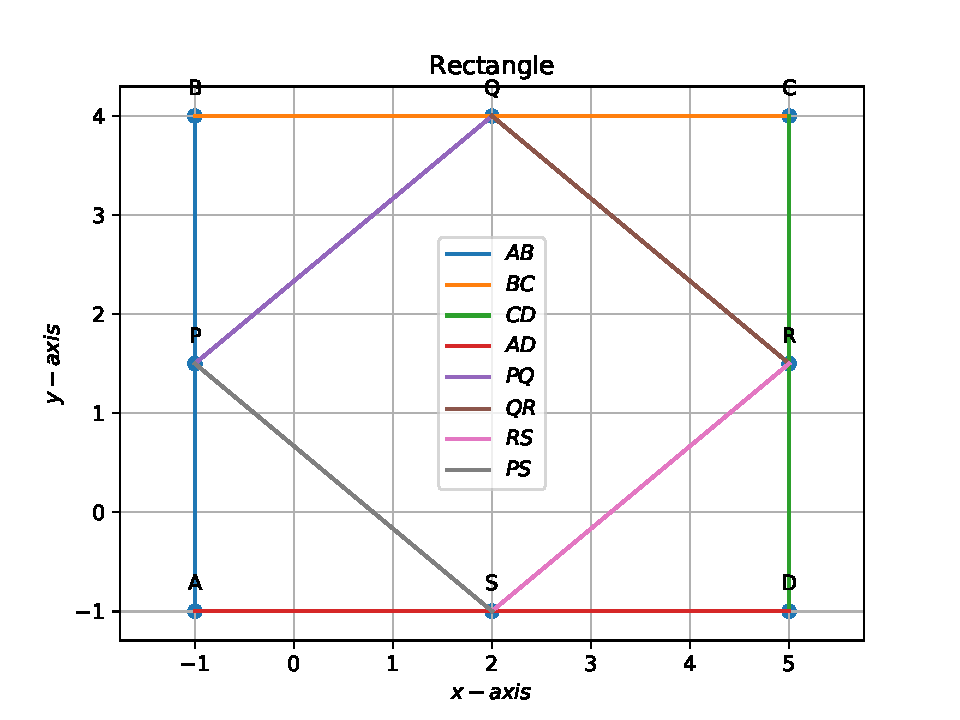
\includegraphics[width=\columnwidth]{chapters/10/7/4/8/figs/problem1.pdf}
	\end{center}
\caption{}
\label{fig:10/7/4/8Fig3}
\end{figure}
We know that PQRS is a parallelogram. To know, if it is a rectangle, we need to ascertain whether any of the two adjacent sides are perpendicular. 
That means $\brak{\vec{Q}-\vec{P}}^\top\brak{\vec{R}-\vec{Q}}$ should be equal to zero. 
\begin{align}
\vec{Q}-\vec{P} &=  \myvec{
 2 \\
 4 \\
 } - \myvec{
 -1 \\
 \frac{3}{2} \\
 } = \myvec{
 3 \\
 \frac{5}{2} \\ 
 } \\
 \vec{R}-\vec{Q} &=  \myvec{
 5 \\
 \frac{3}{2}\\
 } - \myvec{
 2 \\
 4 \\
 } = \myvec{
 3 \\
 -\frac{5}{2} \\ 
 } \\ 
 \brak{\vec{Q}-\vec{P}}^\top\brak{\vec{R}-\vec{Q}} &= \myvec{
 3 & \frac{5}{2}} \myvec{
 3 \\
 -\frac{5}{2} 
 } \neq 0
\end{align}
Therefore PQRS is not a rectangle. Let us check if it is a rhombus. For a rhombus, the diagonals bisect perpendicularly. That means $\brak{\vec{R}-\vec{P}}^\top\brak{\vec{S}-\vec{Q}}$ should be equal to zero. 
\begin{align}
\vec{R}-\vec{P} &=  \myvec{
 5 \\
 \frac{3}{2} \\
 } - \myvec{
 -1 \\
 \frac{3}{2} \\
 } = \myvec{
 6 \\
 0 \\ 
 } \\
 \vec{S}-\vec{Q} &=  \myvec{
 2 \\
 -1 \\
 } - \myvec{
 2 \\
 4 \\
 } = \myvec{
 0 \\
 -5 \\ 
 } \\ 
 \brak{\vec{R}-\vec{P}}^\top\brak{\vec{S}-\vec{Q}} &= \myvec{
 6 & 0} \myvec{
 0 \\
 -5 \\
 } = 0
\end{align}
Therefore $PQRS$ is a rhombus.




\end{enumerate}



